\documentclass[twoside,11pt]{article}

\usepackage{blindtext}

% Any additional packages needed should be included after jmlr2e.
% Note that jmlr2e.sty includes epsfig, amssymb, natbib and graphicx,
% and defines many common macros, such as 'proof' and 'example'.
%
% It also sets the bibliographystyle to plainnat; for more information on
% natbib citation styles, see the natbib documentation, a copy of which


% is archived at http://www.jmlr.org/format/natbib.pdf

% Available options for package jmlr2e are:
%
%   - abbrvbib : use abbrvnat for the bibliography style
%   - nohyperref : do not load the hyperref package
%   - preprint : remove JMLR specific information from the template,
%         useful for example for posting to preprint servers.
%
% Example of using the package with custom options:
%
% \usepackage[abbrvbib, preprint]{jmlr2e}

\usepackage[preprint]{jmlr2e}
\usepackage{amsmath}

% Definitions of handy macros can go here

\newcommand{\dataset}{{\cal D}}
\newcommand{\fracpartial}[2]{\frac{\partial #1}{\partial  #2}}

% Heading arguments are {volume}{year}{pages}{date submitted}{date published}{paper id}{author-full-names}

\usepackage{lastpage}
\jmlrheading{23}{2025}{1-\pageref{LastPage}}{1/21; Revised 5/22}{9/22}{21-0000}{Yaoshiang Ho}

% Short headings should be running head and authors last names

\ShortHeadings{Supervised Learning Preference Optimization}{Yaoshiang Ho}
\firstpageno{1}

\begin{document}

\title{Supervised Learning Preference Optimization: Rethinking RLHF and DPO as Supervised Learning}

\author{\name Yaoshiang Ho \email yaoshiang@gmail.com \\
      %  \addr Department of Statistics\\
      %  University of Washington\\
      %  Seattle, WA 98195-4322, USA
      %  \AND
      %  \name Author Two \email two@cs.berkeley.edu \\
      %  \addr Division of Computer Science\\
      %  University of California\\
      %  Berkeley, CA 94720-1776, USA
      }

\editor{}

\maketitle 

\begin{abstract}%   <- trailing '%' for backward compatibility of .sty file
We propose Supervised Learning Preference Optimization (SLPO), 
an approach to aligning language models that relies solely on the
classic supervised learning loss function, cross-entropy. 
Unlike Reinforcement Learning from Human Feedback (RLHF), 
SLPO directly adjusts probability mass for chosen, rejected, 
and other sequences relative to a reference model, 
eliminating the need for KL divergence regularization. 
SLPO also avoids the extensive reparameterization of model outputs 
into scores and the Bradley-Terry model required by 
Direct Preference Optimization (DPO). 
As a result, SLPO is a purely supervised learning approach 
to alignment, free of reinforcement learning concepts. 
We further demonstrate how to efficiently implement
a targeted probability mass for the 
intractably large set of sequences that are neither explicitly 
chosen nor rejected. 

\end{abstract}

\begin{keywords}
  Reinforcement Learning from Human Feedback (RLHF), 
  Direct Preference Optimization (DPO)
\end{keywords}

\section{Introduction}

Alignment is the task of ensuring that the behavior of a
Large Language Model (LLM) is consistent 
with human preferences. 

The alignment approach popularized by the commercial success of ChatGPT was 
Reinforcement Learning from Human Feedback (RLHF), \citep{ouyang2022training}. 
Despite its effectiveness, RLHF requires training a second model, called
a reward model, as well as Proximal Policy Optimization (PPO), resulting in a 
technique that is more complex than the basic supervised learning. It also
requires a Kullback-Leibler (KL) divergence term to regularize the
changes to the LLM during alignment training.

Direct Preference Optimization (DPO) is a simpler approach to alignment
which does not require a secondary reward model. In the paper introducing
DPO, the authors examine the underlying
approach of RLHF and propose
the DPO objective to align the target LLM directly using
maximum likelihood estimation (MLE). 
The key insight from the DPO paper is that an LLM's
outputs can be reparameterized into a reward model using ratios, logs,
and the Bradley-Terry model \citep{bradley1952rank}.

The specific contribution of this paper is to reframe the alignment
phase away from reward modeling entirely and treating it simply as
a pure supervised learning problem by training a model to align to
a directly modified probability distribution. We call this
approach Supervised Learning Preference Optimization (SLPO).

\section{Related Work}

As discussed in the introduction,
the commercial success of GPT3 and ChatGPT popularized RLHF
as an 
alignment technique \citep{ouyang2022training}. To resolve
weaknesses of RLHF, DPO was introduced and has
been used in recent frontier models
like Meta's Llama 3 family of models \citep{Rafailov, llama}.

Following DPO, the space of alignment methods has rapidly expanded.
Given the pace of innovation in this area, 
we refer to a recent comprehensive survey on 
alignment methodologies by \cite{wang2024comprehensivesurveyllmalignment}.

\section{Preliminaries: DPO}

We analyze the DPO objective \cite[Eq. 7]{Rafailov},  
defined by its authors as :

\begin{equation}
  \label{eq:dpo}
  L_\mathrm{DPO}(\pi_\theta; \pi_\mathrm{ref}) =
  \underbrace{
  -\mathbb{E}_{(x, y_w, y_l) \sim D} 
  \log }_{1} 
  \left[ 
    \underbrace{\sigma }_{2}
    \left(
    \underbrace{\beta \log \frac{\pi_\theta(y_w \mid x)}{\pi_\mathrm{ref}(y_w \mid x)}}_{3}
    - \underbrace{\beta \log \frac{\pi_\theta(y_l \mid x)}{\pi_\mathrm{ref}(y_l \mid x)}}_{4} 
    \right)
  \right]
\end{equation}
where
\begin{description}
  \item $\pi_\theta$ is the language model to be aligned,
  \item $\pi_\mathrm{ref}$ is the reference language model,
  \item $D$ is the dataset of training examples,
  \item $x$ is the input context,
  \item $y_w$ is the winning sequence,
  \item $y_l$ is the losing sequence,
  \item $\sigma$ is the sigmoid function,
  \item $\beta$ is a hyperparameter.
\end{description}

In the underbraced section 1, we see the standard 
negative log likelihood (NLL) objective.
In the underbraced section 2, we see the Bradley-Terry model 
\footnote{A ranking method that is mathematically equivalent and perhaps more 
widely understood is the ELO score, used to rank Chess players, 
and, LLMs in the Chatbot Arena \citep{elo1978rating,chiang2024chatbot}. 
Both ELO and Bradley-Terry assign scores to players, and 
pass the difference through a sigmoid function to assess the probability of 
the minued (aka LHS) player of winning and subrahend (aka RHS) player of losing.}.
In the underbraced sections 3 and 4, we see how the 
reference and language model's predictions are reparameterized
into a winning and losing score: they are the 
log of the ratio of the language model to the reference model, for the winning and 
losing completion, respectively. 
This score is later described as the reward function.

The optimization of $y_w$, a sequence of tokens, rather than
a specific token, is a key difference between the alignment phase and
other phases of training an LLM. In particular, the 
pre-training and supervised fine-tuning (SFT) phases 
focuses on next-token prediction. 


With simple algebraic manipulation, we can rewrite this objective as:
\[
  \label{eq:reg}
  L_\mathrm{DPO}(\pi_\theta; \pi_\mathrm{ref}) =
  \underbrace{
  -\mathbb{E}_{(x, y_w, y_l) \sim D} 
  \log }_{1} 
  \left[ 
    \underbrace{\sigma }_{2}
    \left(
    \underbrace{\beta \log \frac{\pi_\theta(y_w \mid x)}{\pi_\theta(y_l \mid x)}}_{3}
    - \underbrace{\beta \log \frac{\pi_\mathrm{ref}(y_w \mid x)}{\pi_\mathrm{ref}(y_l \mid x)}}_{4} 
    \right)
  \right].
\]
We can interpret the undercomponents as follows: 
The first and second underbraces remain unchanged. 
The third underbrace is the log of the ratio
language models probability of the winner divided by the loser. This ratio 
is optimized to be bigger, given that the log, sigmoid, and log from underbraces
1, 2, and 3 are all monotonic functions. Since a ratio of probabilities is
an odds ratio, we will refer to this as the 
language model's \emph{log-odds ratio}. 

The fourth underbrace is reference model's \emph{log-odds ratio}. As
the weights of the reference model are constant during optimization
of the language model, so too are these values. However,
each row of training data will have a different value for this constant. 
More specifically, since $\pi_\theta$ is initialized as $\pi_\mathrm{ref}$, 
the difference between underbraces 3 and 4 starts at zero during training, 
and the shape of the sigmoid function (underbrace 2) and its gradient are
known. During training, as the language model's \emph{log-odds ratio} increases,
the sigmoid function will naturally regularize and decelerate
the increase by reducing the magnitude of the gradient (a 
useful version of the vanishing gradient problem). 
This is the exact outcome described by the DPO authors 
in their analysis of the gradient of DPO. \emph{But we have developed a different
intuition the DPO loss: rather than reparameterizing the language model's
output into a reward model, the DPO objective optimizes the 
language model's log-odds ratio, with a constant shift so that the 
shifted value starts at zero during optimization.}

Let's continue reworking the DPO objective into mathematically
equivalent forms to better understand it by looking at tokens and their logits rather
than sequences \footnote{
  Technically, a logit is the log-odds ratio and it is the output of a 
  feature extractor before a sigmoid activation function in binary
  classification. The term logit is also used for categorical classification,
  when a feature extractor's outputs are 
  activated with the softmax function. However,
  these softmax logits cannot be exponentiated to calculate an odds ratio. 
  They do have an unfortunate property
  however: they are shift invariant, leading to numerical instability and
  the need for log-softmax and its use of the log-sum-exp trick to improve
  numerical stability. In this paper, since we are dealing
  with both sigmoid and softmax functions, we will refer to the value
  passed into a softmax function as a softmax logit.
}. 

The variable $y$ is a sequence of tokens, defined as

\begin{equation}
  \label{eq:joint}
  \pi_\mathrm{ref}(y \mid x) = \prod_{t=1}^T \pi_\mathrm{ref}(y_t \mid x, y_{<t}),
\end{equation}
where 
\begin{description}
\item \(y = (y_1, y_2, \ldots, y_T)\) is the output sequence,
\item \(x\) is the input context, and
\item \(y_{<t} = (y_1, y_2, \ldots, y_{t-1})\) represents the tokens 
  generated prior to time step \(t\). 
\item 
\(\pi_\mathrm{ref}(y_t \mid x, y_{<t})\) denotes the conditional 
probability of generating token \(y_t\) given the input \(x\) and 
the previously generated tokens \(y_{<t}\).
\end{description}

Since both $\pi$ language model are LLMs, they are activated
using the softmax function. 
The softmax operation can be mathematically cumbersome 
due to its dependence on all other logits for normalization. 
For simplicity, we assume that the logits are transformed 
using a log-softmax function, which computes the logarithm 
of the softmax probabilities in a numerically stable way. 
This transformation results in log-probs, 
which are easier to reason about since they 
can be exponentiated to recover probabilities. 
Importantly, we do not lose any generality because 
log-probs can also be passed through a softmax 
function to recover probabilities, ensuring equivalent behavior.

Let us establish the term $\mathrm{f}$ for the layers of the model up to the softmax
activation, namely, the feature extractor which outputs logits. The output of 
$\mathrm{g}$ are logprobs, which are a special case of logits: they
can be converted to the probability distribution function using 
either softmax or exponentiaion. 

\begin{equation}
  \label{eq:g}
  \mathrm{g}(y \mid x) = \mathrm{logsoftmax}(\mathrm{f}(y \mid x))
\end{equation}
such that
\[
  \pi(y \mid x) = \exp (\mathrm{g}(y \mid x)) = 
  \mathrm{softmax}(\mathrm{g(y \mid x)}) = \mathrm{softmax}(\mathrm{f(y \mid x)}).
\]
Plugging Equations ~\ref{eq:joint} and ~\ref{eq:g} into the DPO objective ~\ref{eq:dpo}, 
\begin{multline}
  \nonumber
  L_\mathrm{DPO}(\pi_\theta; \pi_\mathrm{ref}) = 
  -\mathbb{E}_{(x, y_w, y_l) \sim D} 
  \log \\ 
  \left[
    \sigma 
    \left(
      \beta \log \frac
      {\prod_{t=1}^{T_w} \exp (\mathrm{g_\theta}(y_{w,t} \mid x, y_w{<t}))}
      {\prod_{t=1}^{T_w} \exp (\mathrm{g_\mathrm{ref}}(y_{w,t} \mid x, y_w{<t}))}
      - 
      \beta \log \frac
      {\prod_{t=1}^{T_l} \exp (\mathrm{g_\theta}(y_{l,t} \mid x, y_w{<t}))}
      {\prod_{t=1}^{T_l} \exp (\mathrm{g_\mathrm{ref}}(y_{l,t} \mid x, y_w{<t}))}
      \right)
      \right]
    \end{multline} 
which simplifies to: 
\begin{multline}
  L_\mathrm{DPO}(\pi_\theta; \pi_\mathrm{ref}) = 
  -\mathbb{E}_{(x, y_w, y_l) \sim D} 
  \log \\ 
  \left[
    \sigma 
    \left(
      \beta 
        \left( 
          \sum_{t=1}^{T_w} \left[ \mathrm{g_\theta}(y_{w,t} \mid x, y_{w,<t}) - \mathrm{g_\mathrm{ref}}(y_{w,t} \mid x, y_{w,<t}) \right] 
          -
          \sum_{t=1}^{T_l} \left[ \mathrm{g_\theta}(y_{l,t} \mid x, y_{l,<t}) - \mathrm{g_\mathrm{ref}}(y_{l,t} \mid x, y_{l,<t}) \right] 
        \right)
    \right)
  \right]
\end{multline}

We notice another possibility to rewrite the DPO objective towards something
more familiar. Optimizing the sigmoid of a difference $a-b$ through BCE 
is equivalent to optimizing the softmax of $a$ and $b$ through CCE towards 
a one-hot encoded target of $y_\mathrm{true} = [1, 0]$. 
This is well known
but derived in Appendix~\ref{app:ce-of-diff-same-as-softmax}. This allows
us to rewrite the DPO objective as follows:

\begin{equation}
\label{eq:dpo-as-cce}
L_\mathrm{DPO}(\pi_\theta; \pi_\mathrm{ref}) = 
-\mathbb{E}_{(x, y_w, y_l) \sim D} \, 
\text{CCE}
\left[
  y_\mathrm{true} = 
    \begin{bmatrix}
    1 \\ 
    0
    \end{bmatrix}
  ,
  y_\mathrm{pred} = 
    \text{softmax}
    \left(
    \begin{bmatrix}
    \beta S_w \\ 
    \beta S_l
    \end{bmatrix}
  \right)
\right]
\end{equation}
where
\begin{description}
\item
$ S_w = 
  \underbrace{
    \sum_{t=1}^{T_w} \mathrm{g_\theta}(y_{w,t} \mid x, y_{w,<t}) 
    }_{A}
    \underbrace{
  - 
  \sum_{t=1}^{T_w}\mathrm{g_\mathrm{ref}}(y_{w,t} \mid x, y_{w,<t})
  }_{B}
$
\item
$
S_l = 
  \underbrace{
    \sum_{t=1}^{T_l} \mathrm{g_\theta}(y_{l,t} \mid x, y_{l,<t}) 
  }_{A}
  \underbrace{
  - 
  \sum_{t=1}^{T_l} \mathrm{g_\mathrm{ref}}(y_{l,t} \mid x, y_{l,<t})
  }_{B}
$
\end{description}

\paragraph{Key Observation \#1: Much of the DPO objective 
can be simplified to the form of a 
standard classification task.} \label{obs:dpo-as-cce}
Equation~\ref{eq:dpo-as-cce} 
provides our first key observation. 
What started off as a complex reparameterization 
of the language model's output into a reward
model and a Bradley-Terry model, 
has been simplified into a standard 
categorical crossentropy loss applied to the softmax, with
simple to understand targets. However, the
input to the softmax is not a single logit, but rather, the 
summation of all the winning (or losing) logits in the language model
(underbraces A), 
subtracted by the same summation from the reference model (underbraces B).
Our next two observations will interpret those. 

\paragraph{Key Observation \#2: The difference terms simply zero-align
the input to the softmax function across all examples during training,
allowing the training to equally optimize all examples.} 
Since
the language model is initialized by the reference model,
the difference introduced in underbraces B of Equation~\ref{eq:dpo-as-cce}
simply zero-aligns
the input to softmax, allowing the training process to send identical
gradients to all examples, regardless of the relative probabilities
$\mathrm{\pi}(y_w)$ and $\mathrm{\pi}(y_l)$ for that example. 
This difference is the
vestige of underbraces 3 and 4 in the original DPO objective in 
Equation~\ref{eq:dpo}
was refered to as a "reward function", 
but we now consider it simply a zero-aligning of examples. We have
successfully eliminated reinforcement learning concepts from the DPO objective. 


\paragraph{Key Observation \#3: DPO optimizes a joint probability}
The summation in unbraces A of Equation~\ref{eq:dpo-as-cce}
may not be familiar. In fact, the softmax of a sum optimizes a joint probability.
See Appendix~\ref{app:softmax-sum-joint}
for a derivation. 
This should not be surprising since the original DPO objective 
optimizes the joint probability of the winning and losing sequences. 
Equation~\ref{eq:joint} expresses this as the joint probability of 
tokens, represented as a product, and a product of 
probabilities is equivalent to a sum of log probabilities.

\paragraph{Key Observation \#4: Behind the summations and shifts
in unbraces A and B of Equation~\ref{eq:dpo-as-cce}, 
the final objective is still $+inf$ or $-inf$ for each token logit.} 
This
is obvious from Equation~\ref{eq:dpo-as-cce}. An equivalent statement is that
the DPO objective does not consider any sequence other than the
winning and losing, and if left unchecked, would ultimately force
the model to predict the winning sequence with probability 1 and all
other sequences, including the loser, with probability 0. This is obviously
destabilizing, e.g. other sequences may have been perfectly
reasonable as winning sequences. This is a weakness
of the DPO objective. 

We have been able to remove much of the machinery of the DPO objective 
through algebraic manipulation and equivalences to more common
deep learning concepts.
We have also developed key observations on the strength and weaknesses
of the DPO objective. Can we take these learnings 
and develop a superior objective? 


\section{Preliminaries: Probabilistic Classification}

\begin{figure}[htbp]
  \centering
  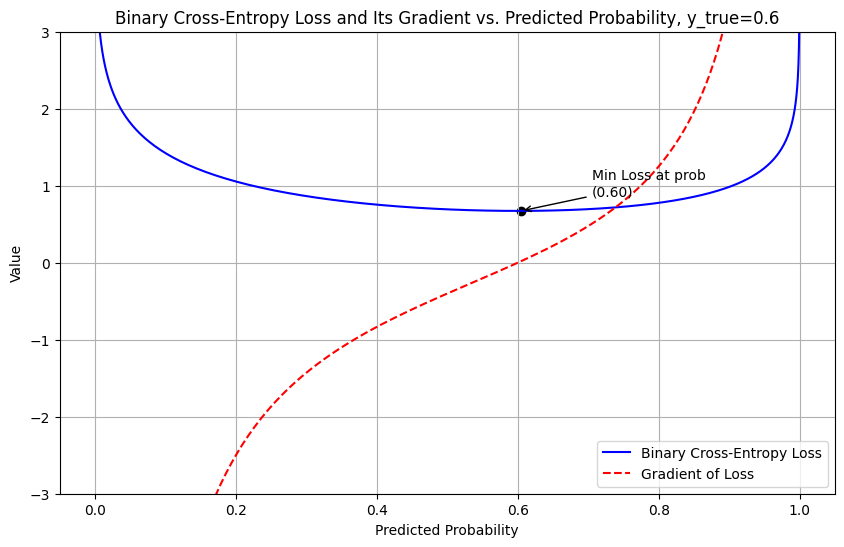
\includegraphics[width=0.8\textwidth]{ce06.png}
  \label{fig:ce06}
  \caption{Setting $y_\mathrm{true}$ to a value 
  other than 0 or 1 is a valid 
  use of the crossentropy loss 
  function and perfectly consistent with
  both KL divergence and MLE.}
\end{figure}

A basic task for deep learning has been classification, both
binary and categorical. 
\begin{itemize}
\item Look at this image and decide which of the ten digits it is 
  \citep{lecun1998mnist}.
\item Classify every pixel in this image as a foreground class or background. 
\item Decide if this movie review's sentiment is positive or
negative \citep{Pang+Lee:04a}.
\end{itemize}

Modern LLMs auto-regressively predict a probability distribution for 
the next token among a finite set of possibilities, conditioned on the 
previous tokens. Hence, an LLM also solves 
a classification problem. 

Given the prevalence of classification, deep learning oftens assumes
target labels can be described as either ordinal numbers
or equivalently one-hot encoded vectors. When target labels are
intermediate values between one and zero, they were called "soft targets", 
treated as an regularization technique or even called dark knowledge
\citep{hinton2015distilling, szegedy2016rethinking,hinton2014dark}. 

But the two roots of the crossentropy
loss functions, KL divergence and Maximum Likelihood Estimation (MLE) applied
to the probability distribution function of a Multi-Bournoulli
distribution, are not limited to binary and categorical outcomes. 
For example, the crossentropy loss function can be used directly 
to condition a model to predict to be true 60\% of the time and false 40\% of 
the time, as demonstrated in Figure~\ref{fig:ce06}. 

The term we will use for the idea of
predicting a probability distribution is \emph{probabilistic classification}.

\section{Supervised Learning Preference Optimization}

Armed with intuition of the DPO loss and probabilistic classification, we can
now turn to a simpler, supervised learning approach to alignment. Our
goals are:
\begin{itemize}
\item Apply only MLE under a probabilistic classification approach. 
  That is, we only want to use a CCE loss function. 
\item Avoid any RL concepts like rewards.
\item Avoid any extra ratios, logs, or the Bradley-Terry model.
\item Continue optimizing sequences rather than individual tokens.
\item Continue giving comparable weight to all examples during optimization.
\item Continue stabilizing the optimization to prevent divergence.  
\item Instead of having an unconstrained objective, 
  specify an objective with a natural "bowl shape" at a target, to assist
  in optimization.
\end{itemize} 

The SLPO objective achieves these goals
by directly optimizing probablities for the winning, losing,
and all other sequences. It is defined as follows:

\begin{align}
  \label{eq:slpo}
  L_\mathrm{SLPO}(\pi_\theta; \pi_\mathrm{ref}) =
  -\mathbb{E}_{(x, y_w, y_l) \sim D} &\Bigg(
    \underbrace{
      w_w \cdot \log \pi_\theta(y_w \mid x)
    }_{1} \notag \\
    &\quad +
    \underbrace{
      0 \cdot \log \pi_\theta(y_l \mid x)
    }_{2} \notag \\
    &\quad +
    \underbrace{
      (1 - w_w) \cdot \log \pi_\theta(y_{\overline{w \cup l}} \mid x)
    }_{3}
  \Bigg)
\end{align}
where 
\begin{description}
  \item $x$ is the input context,
  \item $y_w$ is the winning token sequence,
  \item $y_l$ is the losing token sequence,
  \item $\pi_\theta$ is the language model to be aligned,
  \item $\pi_\mathrm{ref}$ is the reference language model,
  \item $w_w = \pi_\mathrm{ref}(y_w \mid x) + \pi_\mathrm{ref}(y_l \mid x)$, and
  \item $y_{\overline{w \cup l}}$ represents all other possible token sequences.
\end{description}

Intuitively, the goal is to take the probabilities of the winning
and losing sequence and reallocate them to the winning sequence (underbrace 1).
The losing sequence is optimized to zero probability (underbrace 2). 
Importantly,
the other tokens are directly optimized to maintain 
the same probability as the reference model  (underbrace 3). 
This is essentially the SLPO's version of
the KL divergence regularization term in traditional RLHF. 

Alternatively, a softer version of the SLPO objective 
would shift the probabilities in a probabilistic matter: 
\begin{align}
  L_\mathrm{SLPO}(\pi_\theta; \pi_\mathrm{ref}) =
  -\mathbb{E}_{(x, y_w, y_l) \sim D} &\bigg(
    w_w \cdot \log \pi_\theta(y_w \mid x)  \notag \\
    &+ w_l \cdot \log \pi_\theta(y_l \mid x)  \notag \\
    &+ (1 - w_w - w_l) \cdot \log \pi_\theta(y_{\overline{w \cup l}} \mid x)
  \bigg)
\end{align}
where
\begin{description}
  \item $w_w = \alpha \cdot \left( \pi_\mathrm{ref}(y_w \mid x) + \pi_\mathrm{ref}(y_l \mid x) \right)$, 
  \item $w_l = (1 - \alpha) \cdot \left( \pi_\mathrm{ref}(y_w \mid x) + \pi_\mathrm{ref}(y_l \mid x) \right)$, and
  \item $0.5 < \alpha <= 1.0$.
\end{description}

\section{Implementation}

For a standard language model, the vocabulary size $v$ is typically in the range
of 10,000 to 100,000 tokens. The sequence length $T$ is typically
in the range of 128 to 1024 tokens. 
So the $y_{\overline{w \cup l}}$ set of sequences is intractably large to 
enumerate. 

Let us consider $y_w$ independently of $y_l$. Then we can rewrite
the SLPO Equation~\ref{eq:slpo} in two halves and consider them separately:

\begin{align}
  \nonumber
  \label{eq:slpo-equiv}
  L_\mathrm{SLPO}(\pi_\theta; \pi_\mathrm{ref}) =
  -\mathbb{E}_{(x, y_w, y_l) \sim D} 
  &\Bigg(
  \underbrace{
      w_w \cdot \log \pi_\theta(y_w \mid x)
    }_{1}
    + 
    \underbrace{
      (1 - w_w) \cdot \log \pi_\theta(y_{\overline{w}} \mid x)
    }_{2} \notag \\
  &\quad +
  \underbrace{ 
      0 \cdot \log \pi_\theta(y_l \mid x)
    }_{3}
      + 
      \underbrace{ 
        1 \cdot \log \pi_\theta(y_{\overline{l}} \mid x)
      }_{4}
  \Bigg)
\end{align}

The term focused on the winning sequence (underbrace 1) is simple: 
it is just the sum of the logits of the winning token sequences, passed
through softmax and CCE with the target weight. 

For the term focused on the losing sequence (underbrace 3), the loss at 
every token position is also simple: like underbrace 1, we sum the logits
before we pass them into softmax 
and assign a target value of zero in the CCE loss. 
The terms in underbrace 2 and underbrace 4 are the tricky ones, since
they deal with complementary sets.
However, we can see a recursive 
pattern by visualizing a tree. For the first position in the sequence, there 
are essentially two options: 
the winning token (or losing token) and everything else. 
The target odds of everything else is simply
\( 1 - w_w \), and the predicted odds is the 
\[
\sum \exp\left(\mathrm{logsoftmax}(z_{\overline{w}})\right).
\]
Obviously, we can calculate
this with the logsumexp trick for both numerical stability and to stay in 
log space.
Importantly, \emph{we do not need to recursively explore sequence
position 2 and beyond for sequences that start with a non-winning token}. 

Similarly, for position 
two, we can directly calculate the predicted probability as 
\[
\pi_\theta(y_{w, 1}) \cdot \pi_\theta(y_{\overline{w}, 2}).
\]
Adding all such terms to our running total results in 
\[
\log \pi_\theta(y_{\overline{w}} \mid x),
\]
which we compute efficiently in a vectorizable way. 

Formally, the term \(\log \pi_\theta(y_{\overline{w}} \mid x)\) is calculated as:
\[
\log 
\sum_{j=1}^{T} 
  \pi_\theta(y_{\overline{w},t} \mid y_{w:t-1}, x)
\prod_{k=1}^{j} 
  \pi_\theta(y_{w,k} \mid x, y_{w:<k}).
\]


\subsection{Code}

An implementation of the SLPO objective on a single sequence 
is provided below. Additional utility functions for generating
datasets available at \url{https://github.com/yaoshiang/rlhf-mle}.

\begin{verbatim}
  from typing import Tuple, Dict, List

  import torch
  
  from torch import Tensor
  
  from torch.nn import functional as F
  from torch.nn.modules.loss import _Loss
  
  
  def _compute_logprob_y_bar_y(
      logprobs: torch.Tensor, y_tokens: torch.Tensor
  ) -> Tuple[torch.Tensor, torch.Tensor]:
      """
      Given:
        logprobs: shape (T, V) = log softmax outputs for a single sequence.
        y_tokens: shape (T,) = sequence of token-IDs.
  
      Returns:
        (log_p_y, log_p_not_y):
  
        Where:
          log_p_y = log probability of exactly matching y_tokens.
          log_p_not_y = log probability of any sequence that differs
                        from y_tokens in at least one position.
      """
      T, _ = logprobs.shape  # T = sequence length, _ = vocab size
  
      # Logprobs should sum to log(1.0) = 0.0 for each time step t.
      logprob_t = torch.logsumexp(logprobs, dim=-1)
      assert torch.allclose(logprob_t, torch.zeros_like(logprob_t), atol=1e-3)
  
      # Edge case: Handle empty sequences
      if T == 0:
          raise ValueError("Empty sequences are not supported.")
  
      # 1) Extract log probability of the chosen tokens
      logprob_y_t = logprobs[torch.arange(T), y_tokens]
      logprob_y = logprob_y_t.sum()  # Log of joint prob of y seq over steps t.
  
      # 2) Compute sigma sums for "first mismatch" trick
      logprob_sigma_y_lt_t_shifted = torch.cat(
          [
              torch.tensor(
                  [0.0], device=logprobs.device, dtype=logprobs.dtype
              ),  # Initial zero for sigma sum
              torch.cumsum(logprob_y_t, dim=0),  # Shape (T)
          ]
      )  # Shape (T+1)
      logprob_sigma_y_lt_t = logprob_sigma_y_lt_t_shifted[:-1]  # Shape (T,)
      del logprob_sigma_y_lt_t_shifted  # Free memory
  
      assert logprob_sigma_y_lt_t.size() == (T,)
  
      # 3) Compute log probability of any incorrect token at each step
      # Better to not use torch.log1p(-torch.exp(logprob_y_t)).
      # Uncertain if the gradients will be correct with that shortcut
      # given log_softmax layer. Instead, clone and mask y_t to -inf.
      # logsumexp will handle -inf values correctly.
      logprob_masked_y_t = logprobs.clone()
      logprob_masked_y_t[torch.arange(T), y_tokens] = -float("inf")
      logprob_bar_y_t = torch.logsumexp(logprob_masked_y_t, dim=-1)
  
      # 5) Compute the mismatch log probability
      logprob_not_y = torch.logsumexp(
          logprob_sigma_y_lt_t + logprob_bar_y_t, dim=0
      )
  
      return logprob_y, logprob_not_y
  
  
  def slpo_loss(input: torch.Tensor, target: dict) -> torch.Tensor:
      r"""Calculates the SLPO loss for a single sequence:
          w_w * log p_theta(y_w)
          + (1 - w_w) * log p_theta(\overline{y_w})
          + 0 * log p_theta(y_l)
          + 1 * log p_theta(\overline{y_l})
  
      Args:
          input: Float tensor of shape (T, V).
                 Raw logits from the LM for each batch element n,
                 each time-step t, each vocab token v.
          target: A dict with entries:
              - 'pi_ref_w': scalar tensor, float. Ref prob for winning/chosen seq.
              - 'pi_ref_l': scalar tensor, float. Ref prob for losing/rejected seq.
              - 'y': shape (T), tensor, int. The winning/losing token IDs.
              - 'winner': scalar, tensor, bool. True means winner/chosen, False means
                  loser/rejected.
  
      Returns:
          A scalar Tensor.
      """
      # Checks
      assert input.dim() == 1, f"Expected 1D input, got {input.dim()}"
      assert input.size() == target["y"].size(), (
          f"Expected input and target to have the same size, got "
          f"{input.size()} and {target['y'].size()}"
      )
  
      # Convert to log-probs
      logprobs = F.log_softmax(input, dim=-1)  # shape (T, V)
  
      if target["winner"]:
          w_w = target["pi_ref_w"] + target["pi_ref_l"]
  
          # Get p_theta(y_w) and p_theta(\overline{y_w})
          log_p_y, log_p_bar_y = _compute_logprob_y_bar_y(logprobs, target["y"])
          loss = -(w_w * log_p_y + (1.0 - w_w) * log_p_bar_y)
      else:
          # Get p_theta(y_l) and p_theta(\overline{y_l})
          log_p_y, log_p_bar_y = _compute_logprob_y_bar_y(logprobs, target["y"])
          loss = -(0.0 * log_p_y + 1.0 * log_p_bar_y)
  
      return loss
  
\end{verbatim}

\section{Future Work}

Most importantly, for future work we will follow the
experimental setup outlines by \cite{Rafailov} to compare the 
relative performance of SLPO against DPO.

We will also explore custom loss functions that can bypass the autograd
of PyTorch, since much of the reasoning behind the SLPO objective
was in the gradient space, and only brought back into loss
space for implementation. 

\section{Conclusion}

In this paper, we have analyzed the DPO objective, found 
its strengths and weaknesses, and proposed a new objective
that is a pure supervised learning approach to alignment.

Given the fact that DPO appeared to be superior to RLHF, if
either a formal proof or empirical experiments can prove that 
the SLPO is superior to DPO, we would consider whether
Reinforcement Learning concepts were ever necessary in alignment. 

% Acknowledgements and Disclosure of Funding should go at the end, before appendices and references

% \acks{The author thanks Chiara Cerini for her
% invaluable reviews of of this work.}

% Manual newpage inserted to improve layout of sample file - not
% needed in general before appendices/bibliography.

\newpage

\appendix

% [appendix]


\section{Equivalence of Cross-Entropy on Sigmoid of Difference
and Categorical Cross-Entropy on Softmax for Two Classes}

\label{app:ce-of-diff-same-as-softmax}

Logistic regression uses 
a single logit \(\alpha\), transforming it through the \emph{sigmoid} function to obtain 
a probability \(\sigma(\alpha) = \frac{1}{1 + e^{-\alpha}} \). The \emph{binary cross-entropy} 
(BCE) loss for a label $y$ and predicted probability \(\hat{y} = \sigma(\alpha)\) is:
\[
  \text{BCE}(y, \hat{y})
  \;=\;
  - \left[
      y \,\log(\hat{y})
      \;+\;
      (1 - y)\,\log (1 - \hat{y})
    \right].
\]

Alternatively, single-label multiclass classification of two 
outcomes uses two softmax logits \(z_1\) and \(z_2\) (one per class) 
and applies the softmax function to obtain probabilities:
\[
  p(y=1 \mid z_1, z_2)
  \;=\;
  \frac{e^{z_1}}{e^{z_1} + e^{z_2}},
  \qquad
  p(y=2 \mid z_1, z_2)
  \;=\;
  \frac{e^{z_2}}{e^{z_1} + e^{z_2}}.
\]
The associated categorical cross-entropy (CCE) loss is: 
\[
  \text{CCE}(y, \hat{y})
  \;=\;
  -\sum_{k=1}^2 y_k \,\log (\hat{y}_k ),
\]
where \(\hat{y}_1 = \frac{e^{z_1}}{e^{z_1} + e^{z_2}}\), 
\(\hat{y}_2 = \frac{e^{z_2}}{e^{z_1} + e^{z_2}}\), 
\(y_1 = 1\), and
\(y_2 = 0\). 

If we set 
\[
  \alpha = z_1 - z_2,
\]
then
\[
  \frac{e^{z_1}}{e^{z_1} + e^{z_2}}
  =
  \frac{1}{1 + e^{z_2 - z_1}}
  =
  \sigma(\alpha).
\] 
Therefore, the predicted probability $\hat{y_1}$ from softmax
matches the \(\sigma(\alpha)\) in logistic regression. This means that 
the BCE loss on the sigmoid of a difference of two numbers ($z_1 - z_2$) 
is equivalent
to the CCE loss on the softmax of the first class
($z_1$) \citep{Goodfellow-et-al-2016}.


\section{Softmax as a sum as a joint probability}
\label{app:softmax-sum-joint}

We prove this for the special case of two examples, each with $N$ 
possible classes, where softmax probabilities are given by:

\[
\hat{y}_j^1 = \frac{e^{z_j^1}}{\sum_{m} e^{z_m^1}}, \quad \hat{y}_k^2 = \frac{e^{z_k^2}}{\sum_{n} e^{z_n^2}}
\]

The joint probability of selecting class $j$ for the first example and class $k$ for the second is:

\[
P(j, k) = \hat{y}_j^1 \hat{y}_k^2
\]

We define the target joint probability as:

\[
y_{\text{true}, j, k} 
= 
C, \quad \sum_{(m,n) \neq (j,k)} y_{\text{true}, m, n} = 1 - C.
\]

We aim to show that the cross-entropy loss:

\[
L = - C \log (\hat{y}_j^1 \cdot \hat{y}_k^2) - (1 - C) \log (\Omega)
\]

where $\Omega$ represents all other possible outcomes, 
a set with cardinality $C^2 - 1$.

can be rewritten as the categorical cross-entropy of a softmax over two terms.

Define the logits for two terms:
\begin{align}
  \nonumber
  s_1 &= \log \hat{y}_j^1 + \log \hat{y}_k^2 = z_j^1 - \log \sum_m e^{z_m^1} + z_k^2 - \log \sum_n e^{z_n^2}, \\
  \nonumber
  s_2 &= \log (\Omega).
\end{align}

Applying the softmax function to these logits:

\[
p_1 = \frac{e^{s_1}}{e^{s_1} + e^{s_2}}, \quad p_2 = \frac{e^{s_2}}{e^{s_1} + e^{s_2}}.
\]

Since $e^{s_1} = \hat{y}_j^1 \hat{y}_k^2$ and $e^{s_2} = \Omega$, we obtain:

\[
p_1 = \frac{\hat{y}_j^1 \hat{y}_k^2}{\hat{y}_j^1 \hat{y}_k^2 + \Omega}, \quad
p_2 = \frac{\Omega}{\hat{y}_j^1 \hat{y}_k^2 + \Omega}.
\]

The categorical cross-entropy loss with target distribution $[C, 1 - C]$ is:

\begin{align}
  \nonumber
  L &= - C \log p_1 - (1 - C) \log p_2 \\
  \nonumber
  &= - C \log \left( \frac{\hat{y}_j^1 \hat{y}_k^2}{\hat{y}_j^1 \hat{y}_k^2 + \Omega} \right) 
        - (1 - C) \log \left( \frac{\Omega}{\hat{y}_j^1 \hat{y}_k^2 + \Omega} \right).
\end{align}

Expanding the logarithms:

\begin{align}
  \nonumber
  L &= - C \left( \log (\hat{y}_j^1 \hat{y}_k^2) - \log (\hat{y}_j^1 \hat{y}_k^2 + \Omega) \right) \\
    \nonumber
    &\quad - (1 - C) \left( \log (\Omega) - \log (\hat{y}_j^1 \hat{y}_k^2 + \Omega) \right) \\
    \nonumber
    &= - C \log (\hat{y}_j^1 \hat{y}_k^2) - (1 - C) \log (\Omega) .
  \end{align}


Thus, we have rewritten the original loss function as the categorical cross-entropy of a softmax over two terms:

\[
L = \text{CCE}(\text{softmax}([s_1, s_2]), y_{\text{true}}=[C, 1 - C]).
\]



\section{Approximate Equivalence of Softmax of Sum and Temperature Scaling}
\label{app:softmax-sum-temp}

\begin{figure}[htbp]
  \centering
  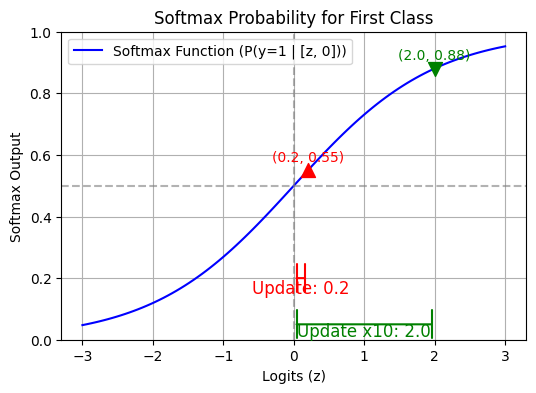
\includegraphics[width=0.8\textwidth]{temperature_grad.png}
  \label{fig:temperature_grad}
  \caption{
    The red update represent the actual update to a logit. But on the next
    itertion of backprop, the gradient is not calculated based on the sigmoid of 
    logit itself, but the sigmoid of the sum of the logit and nine others,
    which we assume to be approximately equal. This pushes the gradient
    calculation out to a less steep part of the curve. This "step function"
    like behavior is similar to a low temperature scaling of a logit
    during training. 
  }
\end{figure}

Here we show that the two-class softmax of a sum of inputs $\alpha_0..\alpha_T$, 
holding 
all other inputs constants, is appromixated by 
temperature scaling, under simplifying assumptions:

\begin{itemize}
  \item We consider the case where the first class is true and the second class is false. 
  \item we assume the output of softmax is passed to Categorical Crossentropy (CCE) loss. 
  \item We assume the second logit to the softmax is zero.
  \item We assume the inputs are approximately equal to each other. 
  \item We assume the many inputs, such as 100. 
\end{itemize}

The softmax of the sum of T inputs is:

\[
  \text{softmax}(
                 [\alpha_1 + \alpha_2 + \ldots + \alpha_T, 0])
  = 
  \frac{e^{\alpha_1 + \alpha_2 + \ldots + \alpha_T}}{e^{\alpha_1 + \alpha_2 + \ldots + \alpha_T} + e^0}
\]

The gradient of the softmax function with a CCE loss is well known to be:
\[
  \frac{\partial \text{CCE}}{\partial z_i} = \hat{y_i} - y_i.
\] 
Equivalently, since $\hat{y_i}$ is the softmax of the sum of the inputs,
\[
  \frac{\partial \text{CCE}}{\partial z_i} = \text{Softmax}(z_i) - y_i,
\] where $z_i$ is the input to softmax. 
Applying this to our unusual softmax of a sum formulation by setting 
$z_i = \sum_{i=1}^T \alpha_i$:
\[
  \frac{\partial \text{CCE}}{\partial z_i} = \text{Softmax}([\sum_{i=1}^T \alpha_i, 0]) - y_i.
\] The nuance here is that due to the chain rule, the gradient on the 
sum of the inputs is passed to each input independently. This is the heart 
of the "multiplication" effect which we will soon see is equivalent to temperature scaling.
For every input $\alpha_k$, the gradient is:
\[
  \frac{\partial \text{CCE}}{\partial \alpha_k} = \text{Softmax}([\sum_{i=1}^T \alpha_i, 0]) - y_i.
\]
But since we assumed all the inputs are approximately equal to each other,
this is equivalent to:
\[
  \frac{\partial \text{CCE}}{\partial \alpha_k} = \text{Softmax}([T \cdot \alpha_k, 0]) - y_i.
\] for all $k$. Rewriting this with the definition of softmax
\begin{equation}
  \label{eq:softmax-sum}
  \frac{\partial \text{CCE}}{\partial \alpha_k} = \frac{e^{T \cdot \alpha_k}}{e^{T \cdot \alpha_k} + e^0} - y_i.
\end{equation} shows a multipler on the input $\alpha_k$ of $T$, representing the cardinality 
of the elements of the sum (e.g. tokens in a sequence). 

Now let's turn to the temperature scaling. The canonical definition of temperature scaling 
per \cite[Equation~2]{hinton2015distilling} is the following, where we use the term
$\mathrm{temp}^{-1}$ to distinguish it from our use of $T$ as the number
of inputs:

\[
\frac{\partial \mathcal{C}}{\partial z_i} = \mathrm{temp}^{-1} \left( 
\frac{e^{z_i \cdot \mathrm{temp}^{-1}}}{\sum_j e^{z_j \cdot \mathrm{temp}^{-1}}} 
- 
\frac{e^{v_i \cdot \mathrm{temp}^{-1}}}{\sum_j e^{v_j \cdot \mathrm{temp}^{-1}}} 
\right)
\] 
where $v_i$ are logits of the teacher and
$z_i$ are the logits of the student. Equivalently:
\[
\frac{\partial \mathcal{C}}{\partial z_i} = \left( 
\frac{e^{z_i \cdot \mathrm{temp}^{-1} - \log(\mathrm{temp})}}{\sum_j e^{z_j \cdot \mathrm{temp}^{-1} - \log(\mathrm{temp})}} 
- 
\frac{e^{v_i \cdot \mathrm{temp}^{-1} - \log(\mathrm{temp})}}{\sum_j e^{v_j \cdot \mathrm{temp}^{-1} - \log(\mathrm{temp})}} 
\right).
\]
Considering we only have two classes, and the second class has a fixed
logit of zero, we can simplify this to:
\[
\frac{\partial \mathcal{C}}{\partial z_1} 
= 
\left( 
\frac{e^{z_1 \cdot \mathrm{temp}^{-1} - \log(\mathrm{temp})}}{e^{z_1 \cdot \mathrm{temp}^{-1} - \log(\mathrm{temp})} + e^{-\log(\mathrm{temp})}} 
- 
\frac{e^{v_1 \cdot \mathrm{temp}^{-1} - \log(\mathrm{temp})}}{e^{v_1 \cdot \mathrm{temp}^{-1} - \log(\mathrm{temp})} + e^{-\log(\mathrm{temp})}} 
\right),
\]
As the logits are optimized up to reasonable non-zero values such as 1.0, 
and with
the assumption that the term $\mathrm{temp}^{-1}$ is large (e.g. the 
number of tokens in a sequence such as 100), 
the terms $\log(\mathrm{temp})$ is dominated
by the term $\mathrm{temp}^{-1}$ and the term . We can replace the terms that use $v$
with $y_i$ since we are using hard targets, not soft labels from a teacher. 
Hence, we can approximate the gradient under KD as

\begin{equation}
\frac{\partial \mathcal{C}}{\partial z_i} = \left( 
  \frac{e^{z_1 \cdot \mathrm{temp}^{-1} }}{e^{z_1 \cdot \mathrm{temp}^{-1} + \mathrm{C}}} 
  - 
y_1
\right)
\end{equation}
where $\mathrm{C}$ is a small constant that is dominated by the term 
$e^{z_1 \cdot \mathrm{temp}^{-1}}$. 
For example, at reasonable values of 
$z_1 = 1.0$ and $\mathrm{temp}^{-1} = 100$, the term 
$e^{z_1 \cdot \mathrm{temp}^{-1}} = e^{100}$, while the term
$e^{-\log(\mathrm{temp})} = 1 / temp = 0.01$. 

This exactly of the form of Equation~\ref{eq:softmax-sum} with the 
temperature scaling term $\mathrm{temp}^{-1}$ replacing the number of inputs 
(such as the number of tokens in a sequence) $T$.
Hence, as optimization proceeds, a softmax of a sum of
many inputs becomes similar to optimizing the softmax of each input with
a low temperature. 

See Figure~\ref{fig:temperature_grad} for an illustration of this concept.




\vskip 0.2in
\bibliography{slpo}

\end{document}
